%        File: chameleon-arch-2.tex
%     Created: Mon Jan 04 08:00 PM 2016 C
% Last Change: Mon Jan 04 08:00 PM 2016 C
%
\documentclass{standalone}

\usepackage{tikz}
\usetikzlibrary{positioning, shapes, calc, backgrounds, fit}

\begin{document}
\begin{tikzpicture}[connection/.style = {<->, blue, line width = 3pt},
  magnify/.style = {dashed, blue, ultra thick}]
  % background: china map
  \node (china-map) [opacity = 0.20] {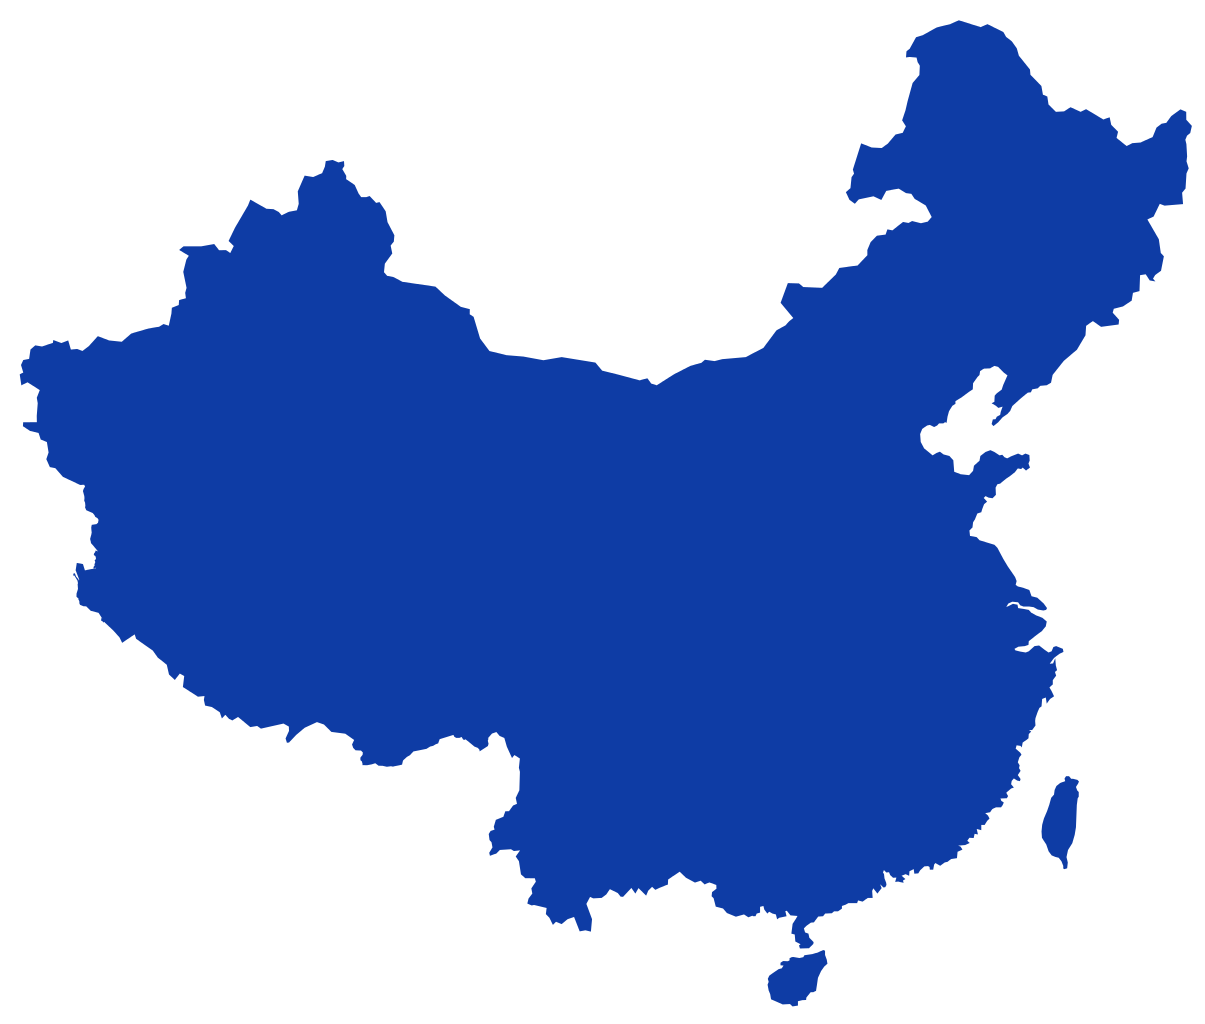
\includegraphics[scale = 0.40]{figs/china-outline-blue.png}};

  % partition-left, partition-right, partition-below
  \node (partition-left) [] at (-6, 1) {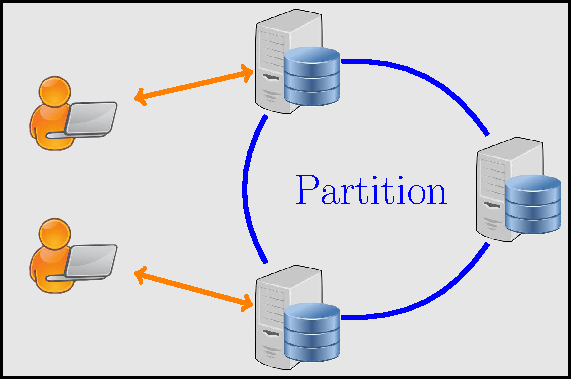
\includegraphics[scale = 0.50]{figs/partition-gray.pdf}}; 
  \node (partition-right) [] at (6, 3) {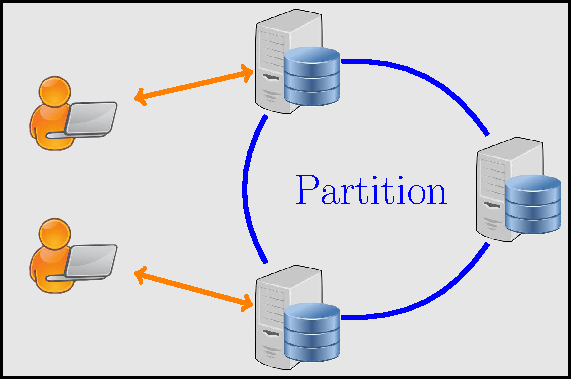
\includegraphics[scale = 0.50]{figs/partition-gray.pdf}}; 
  \node (partition-below) [] at (2, -4) {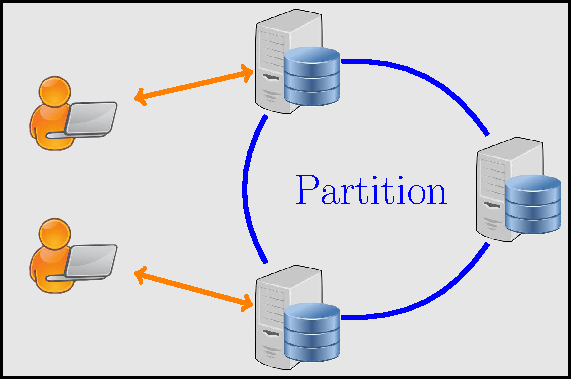
\includegraphics[scale = 0.50]{figs/partition-gray.pdf}}; 

  % connections among partitions
  \draw [connection]  (partition-left) to   (partition-right); 
  \draw [connection] (partition-right) to (partition-below);
  \draw [connection] (partition-below) to (partition-left);

  % replication 
  \node (replication) [font = \LARGE, blue] at (0.5, 0.0) {\textbf{Wide-Area Replication}};
  % magnify partition-left
  \node (partition-magnify) [] at (-6, -5) {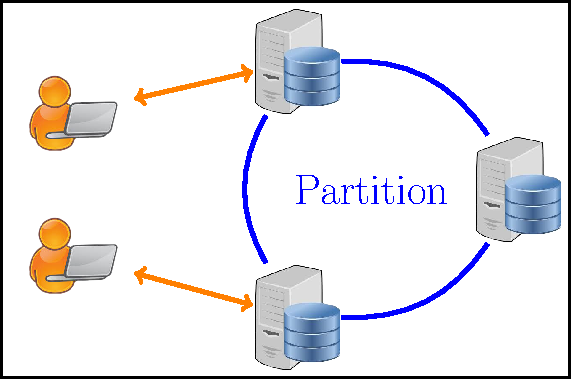
\includegraphics[scale = 0.70]{figs/partition-white.pdf}}; 
  % magnification
  \draw [magnify] (partition-left.south west) to (partition-magnify.north west);
  \draw [magnify] (partition-left.south east) to (partition-magnify.north east);

  % master-slave for one partition
  \begin{scope}[circled/.style = {draw, circle, dashed, ultra thick, red, outer sep = 1pt, minimum size = 1.5cm}, 
    connection/.style = {dashed, red, thick}]
  \node (ms-left) [circled] at (-4, 1) {};
  \node (ms-right) [circled] at (6, 2) {};
  \node (ms-below) [circled] at (4, -4) {};

  \node (master-slave) [below right = 1.5cm and -1.5cm of partition-right] {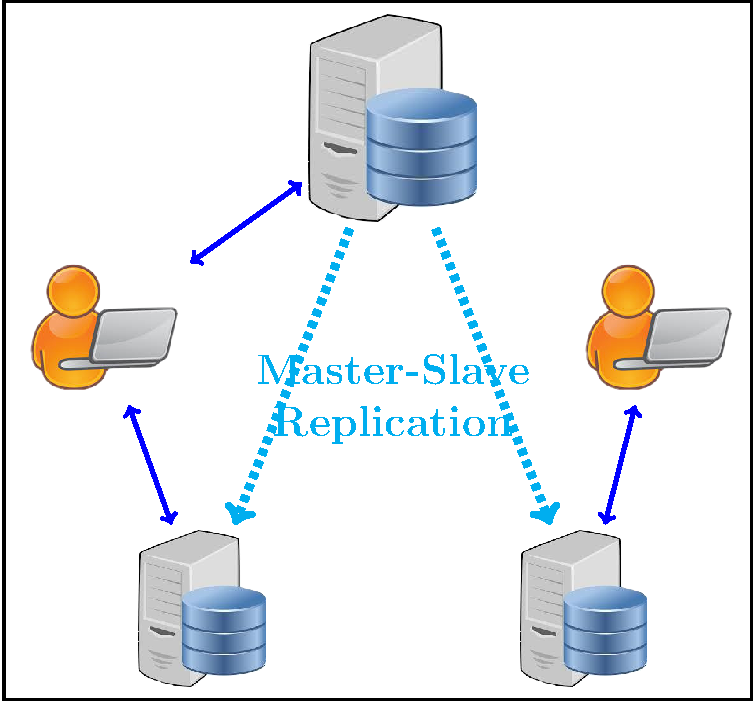
\includegraphics[scale = 0.50]{master-slave.pdf}};
  \draw [connection] (ms-left) to (master-slave);
  \draw [connection] (ms-right) to (master-slave);
  \draw [connection] (ms-below) to (master-slave);
  \end{scope}
\end{tikzpicture}
\end{document}


